\chapter{L'UNIX per i principianti}
Cos'è l'UNIX? Letteralmente, si tratta del nucleo centrale di un sistema operativo
che utilizza la tecnica del time-sharing per gestire le risorse di un calcolatore e distri-
buirle tra i vari utenti. Il sistema consente ai singoli utenti di far girare i propri pro.
grammi, controlla le unità periferiche (dischi, terminali, stampanti e simili) collegate
alla macchina e mette a disposizione un sistema di archiviazione che dà la possibilità
di tenere a lungo in memoria informazioni quali programmi, dati e documenti.\\
In senso più ampio, spesso si intende per UNIX non solo il nucleo centrale, ma an
che i programmi essenziali quali i compilatori, i programmi per le attività di editing\footnote{Per "editing" si 
	intende tutta quella serie di attività legate alla messa a punto redazionale di un testo prima della sua 
	composizione definitiva per la stampa, i comandi di sistema, i programmi di utilità (per la co.
	piatura e la stampa dei file) e così via. [N.d.T.]}
In senso ancora più ampio, l'UNIX può comprendere anche i programmi sviluppa-
ti dagli utenti, come ad esempio quelli per la preparazione dei documenti, routine per
l'analisi statistica e i pacchetti grafici.\\
L'accezione in cui il termine UNIX sarà usato dipenderà da quale livello del sistema sarà preso in considerazione. In questo libro, il contesto chiarirà il significato di
volta in volta.\\
Il sistema UNIX sembra a volte più difficile di quanto non lo sia in realtà, perché
in effetti, per i neofiti, è difficile saper usare in modo ottimale tutte le possibilità che
offre. Fortunatamente, però, non è difficile muovere i primi passi e basta conoscere
alcuni programmi per cominciare a lavorare. Con questo primo capitolo si vuole, nel
più breve tempo possibile, mettervi in grado di usare il sistema. Esso dà una visione
panoramica e non è un manuale; la materia verrà poi in gran parte trattata con maggior
dettaglio nei capitoli successivi.
Gli argomenti principali di questo capitolo sono i seguenti:
\begin{itemize}
	\item attività di base: registrazioni in entrata e in uscita, comandi semplici, correzione
	degli errori di battitura, spedizione della corrispondenza, comunicazioni tra ter-
	minali.
	\item operazioni quotidiane: i file\footnote{Un file è letteralmente un archivio di informazioni/dati.
		In questo testo useremo il termine inglese, comunemente impiegato in informatica). [N.d.T.]} e
	il sistema di gestione relativo, stampa dei file e aree di lavoro, comandi più comunemente usati.
\end{itemize}
Anche se decidete di leggere questo capitolo, vi servirà comunque avere a disposizione
una copia del Manuale di programmazione UNIX; questo perché spesso è più facile
per gli autori rimandarvi al manuale piuttosto che ripeterne i contenuti qui. Questo
libro, infatti, non vuole sostituirsi al manuale, ma intende spiegare come usare al meglio
i comandi in esso descritti. Inoltre, potrebbero esservi delle differenze tra quanto
viene detto in questo testo e la realtà del sistema da voi usato. Il manuale riporta nelle
prime pagine un indice analitico, indispensabile per poter ritrovare i programmi più
adatti per la soluzione dei vari problemi; vi consigliamo di imparare ad utilizzarlo.\\
Infine, un piccolo suggerimento: non abbiate paura degli esperimenti. Sappiate
che, anche se siete dei principianti, sono pochi i possibili casi di errori che potrebbero
incidentalmente nuocere a voi o ad altri utenti. Perciò, cercate di imparare mettendo
in pratica da subito quello che leggete.\\
Questo è un capitolo lungo. Il miglior modo per affrontarlo è di leggerne solo qual
che pagina alla volta esperimentando subito quello che via via imparate.
\section{Come cominciare}
\subsection{ Alcuni prerequisiti a proposito di terminali e di dattilo scrittura}
Onde evitare di spiegare proprio tutto sull'uso dei calcolatori, diamo per scontato che
il lettore abbia famigliarità con i terminali e sappia come usarli. Qualora qualcosa di
quanto viene più avanti esposto vi risulti incomprensibile in base alla vostra esperienza,
vi consigliamo di consultare un esperto del sistema da voi usato.\\
Il sistema UNIX è del tipo definito full duplex, vale a dire che i caratteri battuti sulla
tastiera vengono inviati al sistema che a sua volta li rimanda al terminale perché
vengano scritti a video. Normalmente, questo processo, che ha le caratteristiche
dell'eco, fa sì che i caratteri siano copiati direttamente sul video, rendendo cosi possibile
visualizzare immediatamente ciò che si batte sulla tastiera.\\
A volte, però, come nel caso in cui si debba battere una password (codice di accesso
al sistema) segreta, il processo eco viene temporaneamente sospeso e i caratteri
battuti non appaiono a video. La maggior parte dei tasti riporta normali caratteri alfanumerici;
però, ve ne sono alcuni che servono per dire al calcolatore come interpretare
quanto viene battuto. Di gran lunga il più importante fra questi tasti è quello di
RETURN. Esso è praticamente un codice che segnala la fine di una riga di immissione;
quando incontra questo codice, il sistema risponde posizionando immediatamente
il cursore sul video alla riga successiva. È necessario premere il tasto RETURN perché
il sistema interpreti i caratteri battuti.\\
Tale tasto è perciò un esempio di carattere di comando, vale a dire un carattere in-
visibile che serve a gestire alcuni aspetti di input o di output (immissione/emissione)
sul terminale. Su ogni terminale che si rispetti, per il RETURN esisterà un apposito
tasto; ma per la maggior parte degli altri caratteri di comando non sarà così. Infatti.
perché la macchina li senta, sarà necessario premere contemporaneamente il tasto
CONTROL (spesso abbreviato in CTL o CNTL o anche CTRL) e, a seconda dei casi
un altro tasto, generalmente una lettera dell'alfabeto. Ad esempio, il comando di r
torno si può dare premendo il tasto RETURN o, indifferentemente, premendo con-
temporaneamente CONTROL e la lettera "m''.Il comando RETURN può perciò
anche chiamarsi ``CONTROL - m'' (dal nome dei due tasti) e lo si può scrivere ctl-m
Citiamo qui altri caratteri di comando, per esempio "ctl-d", che serve per dire al pro.
gramma che l'input è terminato; ctrl-g, che fa suonare il campanello del terminale; ctl-h.
chiamato anche ritorno carattere, che può essere usato per correggere gli errori di
battitura; e infine ctrl-i, spesso chiamato tabulatore, per far avanzare il cursore direttamente
alla tabulazione successiva, proprio come sulle normali macchine per scrivere.
Le tabulazioni, sui sistemi UNIX, sono distanziate di 8 caratteri. Sia per il ritorno carattere sia per la tabulazione, esiste un tasto apposito sulla maggior parte dei termi
nali.\\
Vi sono poi altri due tasti che hanno uno speciale significato: il tasto DELETE
(cancella), talvolta chiamato anche RUBOUT o variamente abbreviato, e BREAK
(interruzione) chiamato a volte INTERRUPT. Nella maggior parte dei sistemi
UNIX, premendo il tasto DELETE si provoca l'immediato arresto di un programma
prima che sia finito. In alcuni altri sistemi, tale arresto si ottiene premendo ct/-c. E in
alcuni altri ancora, a seconda di come sono collegati i terminali, BREAK è sinonimo
di DELETE o ct/-c.
\subsection{Un esempio di collegamento in UNIX}
Vediamo di fare un esempio di dialogo tra voi e il vostro sistema UNIX.
In questo testo, ogniqualvolta faremo degli esempi pratici, useremo tre caratteri diversi
che esemplifichiamo: messaggi di sistema, comandi e i testi dell'utente, commenti esplicativi\\
Effettuate il collegamento, sia componendo un numero telefonico oppure girando
un interruttore, a seconda dei casi. Dopo di che sul video dovrebbe apparire quanto
segue:
\begin{description}
	\item[login: nome in codice] \footnote{In questo testo, per convenzione, il vostro nome in codice sarà "alba" e d'ora in poi lo useremo ogniqualvolta necessario. [N.d.T.].} Battete il vostro nome e quindi premete il tasto RETURN
	\item[Password: ] La vostra password (codice di accesso segreto al sistema) non apparirà a video
	mentre la battete
	\item[You have mail: ] Avete della corrispondenza in arrivo. Potrete leggerla dopo aver effettuato le operazioni
	di login
	\item[\$ ] Quando sullo schermo appare il segno del dollaro significa che il sistema è pronto a
	ricevere i vostri comandi
	\item[\$ ] Premete due volte il tasto RETURN
	\item[\$ date] Che data e che ore sono?\\
	{\tt Sunday Sept 25, 23; 02: 57 EDT 1983}
	\item[\$ vho] Chi sta usando la macchina?\\
	\begin{tabular}{llr}
		jib & tty0 & Sep 25 13:59 \\
		alba &tty2 & Sep 25 23:01 \\
		mary & tty4 & Sep 25 19:03 \\
		doug & tty5 & Sep 25 19:22 \\
		egb & tty7 & Sep 25 17:17 \\
		bob & tty8 & Sep 25 20:48
	\end{tabular}
	\item[\$ mail ] Leggete i messaggi\\
	{\tt Da doug Dom 25 Sett 20:53 EDT 1983}\\
	{\tt chiamami quando vuoi lunedì}
	\item[? ] Il comando RETURN fa apparire il
	messaggio successivo
	\item[Da mary - Dom. 25 Sett 19:07 EDT 1983 Si pranza a mezzogiorno domani?] Messaggio successivo
	\item[? d ]  Cancellare questo messaggio
	\item[\$ mail mary ]  Invia messaggio a mary\\
	va bene per il pranzo alle 12
	\item[ctl-d ] Fine messaggi
	\item [\$ ] Chiudete il telefono o spegnete il terminale
	e l'operazione è finita.
\end{description}
A volte ci si può collegare soltanto per leggere dei messaggi, come nel caso sopra indicato, altre volte ci si 
può collegare anche per lavorare. Nella parte rimanente di questo paragrafo prenderemo in esame il 
collegamento sopra descritto, oltre ad alcuni altri programmi che consentono di svolgere attività utili.
\subsection{Operazioni di collegamento}
Dovete in primo luogo farvi assegnare un codice di accesso e una password (codice
accesso segreto: d'ora in poi useremo il termine inglese, comune in ambiente informatico)
dal coordinatore del sistema. L'UNIX è in grado di gestire molti tipi di terminali,
ma è fortemente orientato verso macchine con caratteri minuscoli. La differenza
tra le lettere maiuscole e minuscole è quindi importante con l'UNIX, perciò se il
vostro terminale scrive solo in maiuscolo potreste trovarvi in serie difficoltà e sarebbe
opportuno che vi procuraste un altro tipo di terminale.\\
Assicuratevi che gli interruttori siano nella corretta posizione di lavoro: maiuscolo
o minuscolo, full duplex ed eventuali altre impostazioni iniziali consigliate dal coordinatore:
ad esempio la velocità di linea (cioè il numero di baud). Attivate il collegamento
compiendo il gesto fatato previsto dal vostro terminale: sia esso la composizione
di un numero telefonico o la semplice accensione di un interruttore. Al compi-
mento di tale gesto, a video dovrebbe apparire la scritta login:\\
Se il sistema dovesse inviare altri messaggi sconnessi, potrebbe significare che avete
impostato una velocità sbagliata; controllate quindi la velocità e anche gli altri inter-
ruttori. Se dal controllo risulta che tutto era stato eseguito correttamente, premete al-
cune volte, lentamente, il tasto BREAK oppure INTERRUPT.\\
Se, nonostante tutti questi accorgimenti, non riuscite ad ottenere la scritta login a
video, allora avete bisogno dell'aiuto di un tecnico. Una volta ottenuto login sullo
schermo, battete il vostro codice di accesso in lettere minuscole, e immediatamente
dopo premete RETURN. Se è necessaria la password, il sistema ve la chiederà, però,
come abbiamo già detto, non la farà apparire a video mentre la battete.\\
Dopo che avrete correttamente effettuato le operazioni di accesso, i vostri sforzi
saranno premiati con un messaggio a video, generalmente costituito da un unico carattere,
indicante che il sistema è pronto ad accettare i vostri comandi. Tale messaggio 
può essere costituito dal segno del dollaro (\$) oppure da quello di percentuale (\%)
ma, se volete cambiarlo come meglio preferite vi diremo come fare più avanti. Tale
lettera è in effetti stampata grazie al già menzionato programma interprete, che è
l'interfaccia principale col sistema.\\
Prima del messaggio suddetto, il sistema potrebbe automaticamente stampare la
data, oppure darvi una segnalazione di posta in arrivo. Il sistema vi può anche chiedere
quale tipo di terminale state usando, perché, sapendolo, sarà in grado di utilizzare
al meglio le caratteristiche tecniche del vostro terminale.
\subsection{Comandi di battitura}
Quando il sistema vi segnala di essere pronto (supponiamo con il segno del dollaro (\$)
come sopra citato) potete battere dei comandi, che non sono altro che degli ordini per
il sistema stesso. (Vi segnaliamo che in questo testo useremo il termine programma
come sinonimo di comando). Perciò, quando sullo schermo compare il segno del dollaro
dovete battere "date" (data) e premere il tasto RETURN. Il sistema dovrebbe rispondere
scrivendo la data e l'ora, e dandovi subito dopo un altro segno di dollaro;
per chiarire, tutto quanto sopra descritto sarà visualizzato cosi sul vostro terminale:
\begin{description}
	\item[\$ ] date \\
	{\tt Mon Sep 26 12:20:57 EDT 1983}
	\item[\$ ]
\end{description}
Non dimenticate di premere RETURN e non battete voi il segno del dollaro. Se vede.
te che il sistema è lento a rispondere, premete il tasto RETURN; vedrete che qualcosa
succederà. Attenzione che d'ora in avanti non ripeteremo più di battere il tasto RETURN.
Ricordate però che bisogna premerlo ad ogni fine riga. 
il comando successivo è who (chi) per chiedere chi sono le persone collegate in quel
momento:
\begin{description}
	\item[\$ ] who\\ 
	\begin{tabular}{llr}
		rim & tty0 & Sep 26 11:17 \\
		pjw &tty4 & Sep 26 11:30 \\
		gerard & tty7 & Sep 26 10:27 \\
		mark & tty9 & Sep 26 07:59 \\
		alba & ttya & Sep 25 12:20 \\
	\end{tabular}
	\item[\$ ]
\end{description}
Nella prima colonna è indicato il nome dell'utente. Nella seconda. il nome che il sistema dà al tipo di collegamento usato ("tty" sta per "teletype", un sinonimo arcaico della parola "terminale"). Le restanti colonne danno la data e l'ora del collegamento. Potreste anche provare il seguente comando:
\begin{description}
	\item[\$ who am I ]  (chi sono io?)\\
	{\tt alba ttya Sep 26 12:20}
	\item[\$]
\end{description}
Se, per un errore di battitura, scrivete un comando inesistente, il sistema vi informerà
di non averlo trovato, cosi:
\begin{description}
	\item[\$ whom ]  Testo del comando scorretto (avete scritto
	"whom" al posto di "who")
	\item[whom: not fount] \dots e il sistema ha sapere come gestirlo 
\end{description}
Ovviamente, se per un errore di battitura scrivete il nome di un comando esistente,
che non è quello voluto in quel momento, esso verrà eseguito ugualmente, ma il risultato
non sarà quello desiderato.
\subsection{Comportamento strano del terminale}
Potrà capitare, a volte, che il vostro terminale si comporti in modo alquanto strano:
per esempio, potrebbe stampare ogni lettera due volte oppure, anche premendo il tasto
RETURN, il cursore non si posizionerà a margine della riga successiva. Per ovviare
a questo malfunzionamento è sufficiente spegnere e riaccendere il terminale,
oppure scollegarsi e quindi ricollegarsi. In alternativa, potete anche leggere la descrizione
del comando stty ("set terminal options" : impostare le opzioni del terminale)
al paragrafo 1 del manuale. Se il vostro terminale non ha il tasto per le tabulazioni
potete ottenerle lo stesso battendo il comando:
\begin{description}
	\item[\$ stty -tabs ] 
\end{description}
e il sistema convertirà i caratteri che gestiscono le tabulazioni nell'esatto numero di
spazi da voi voluti. Invece se con il terminale è possibile far impostare le tabulazioni
dal calcolatore, il comando tabs vi consentirà di ottenere i risultati voluti. Perché fun
zioni dovrete magari scrivere:
\begin{description}
	\item[\$ tabs ] tipo di terminale usato 
\end{description}
(Vedere a questo proposito la descrizione del comando tabs nel manuale di programmazione).
\subsection{Errori di battitura}
Se fate un errore di battitura e ve ne accorgete prima di aver premuto il tasto RETURN,
avete due modi per rimediare: potete cancellare i caratteri sbagliati uno alla
volta oppure annullare l'intera riga e ribatterla.
Se battete il carattere per l'annullamento della riga, per default\footnote{Default è un termine comunemente
	usato in ambiente informatico per indicare un comportamento standard 
	del sistema in assenza di istruzioni diverse. [N.d.T.].} il segno @ a esso
farà si che l'intera riga venga eliminata proprio come se non fosse mai stata battuta, e
vi riposizionerà su una nuova riga:
\begin{description}
	\item[\$ ddtae@ ] Riga completamente sbagliata; ricominciare di nuovo
	\item[ date ]  su un'altra riga\\
	{\tt Mon Sep 26 12:23:39 EDT 1983}
	\item[\$ ]
\end{description}
Il segno \# cancella l'ultimo carattere battuto; ogni \# cancella perciò un carattere alla
volta fino ad arrivare all'inizio della riga (ma non va oltre). Così, se fate piccoli errori
di battitura, potete correggerli via via:
\begin{description}
	\item[\$ dd \#atte \#\#e] Correggete via via 
	{\tt Mon Sep 26 12:24:02 EDT 1983}
\end{description}
I segni che provocano la cancellazione dei singoli caratteri o l'annullamento dell'inte.
ra riga sono estremamente dipendenti dal sistema. In molti sistemi (incluso quello che
usiamo noi) quello per la cancellazione dei singoli caratteri è stato sostituito dal tasto
di ritorno carattere e funziona piuttosto bene con i terminali video. Potete veloce.
mente controllare come stanno le cose con il sistema da voi usato nel modo seguente:
\begin{description}
	\item[ datee \textleftarrow ]  su un'altra riga\textleftarrow\\
	{\tt datee \textleftarrow: not found} Il tasto di ritorno non funziona\\ 
	\item[\$ detee \# ] Provate il segno \#\\
	{\tt Mon Sep 26 12:26:08 EDT 1983} È il segno \# quello che va bene
	\item[\$ ]
\end{description}
(Come potete vedere, abbiamo usato il segno - per simboleggiare il ritorno carattere
perché poteste vederlo). Un altro modo molto comune per ordinare l'annullamento
di una riga è quello di battere ct/-u.\\
Nella rimanente parte di questo paragrafo useremo il simbolo \# come carattere di
cancellazione perché è chiaramente visibile. Cercate però di ricordare sempre qual è il
simbolo previsto dal vostro sistema, nel caso fosse diverso. Più avanti, nella parte dedicata 
alla personalizzazione del sistema, vi diremo come fare per usare come simbolo 
di cancellazione carattere o riga il segno che volete una volta per tutte.\\
Cosa fare nel caso in cui il simbolo che serve per il comando di cancellazione carattere,
o annullamento riga, dovesse essere scritto come parte integrante di un testo anziché 
come carattere di comando? Si dovrà semplicemente far precedere i simboli \# e
@ da una barra rovesciata, così:\\
Per inserire quindi in un testo i simboli \# oppure @ con il loro significato originario,
bisognerà battere \textbackslash{} \# o @. A volte capita che il sistema, dopo che avete
battuto il carattere @ preceduto dalla barra rovesciata, faccia comunque avanzare il
cursore del terminale alla riga successiva. Questo non è grave, perché il sistema ha
comunque registrato il segno @ come da voi desiderato.\\
La barra rovesciata, talvolta chiamata "escape character" (carattere di cambio codice),
nella maggior parte dei casi viene usata per indicare che il carattere che la segue
è in qualche modo speciale. Per cancellare tale barra bisogna battere due volte il carattere
di cancellazione, così: \#\#. Vi rendete conto del perché?\\
Dovete sapere che i caratteri battuti, prima di arrivare a destinazione, sono esaminati
ed interpretati da una sequenza di programmi e la loro esatta interpretazione dipende
non solo dal punto d'arrivo, ma anche da come sono giunti a tale meta.\\
Ogni carattere battuto viene immediatamente rimandato, con effetto eco, al terminale,
ad eccezione dei casi in cui l'effetto eco sia stato sospeso, il che è raro. Finché
non viene premuto il tasto RETURN, i caratteri sono temporaneamente memorizzati
dal nucleo centrale del sistema e perciò gli errori di battitura possono essere corretti
con i comandi di cancellazione carattere o annullamento riga. Quando uno dei due
caratteri suddetti è preceduto dalla barra rovesciata, il sistema non prende in considerazione 
la barra e memorizza invece i due simboli senza interpretarli come caratteri di
comando.\\
Quando premete il tasto RETURN, i caratteri memorizzati dal nucleo centrale del
sistema vengono inviati al programma che sta effettuando la lettura dal terminale
Tale programma può, a sua volta, interpretare in modo particolare i caratteri che riceve;
per esempio, l'interprete non assegnerà nessun significato speciale a un carattere
che sia preceduto da una barra rovesciata. Ma riprenderemo questo discorso al capitolo 3.
Per il momento dovete solo ricordare che il nucleo centrale elabora i simboli di cancellazione carattere o annullamento riga, nonché la barra rovesciata, soltanto
se quest'ultima li precede; eventuali caratteri seguenti possono essere interpretati an
che da altri programmi.
\begin{eser}
	Spiegate cosa succede quando a video compare quanto segue:\\
	{\tt \$ date @}
\end{eser}
\begin{eser}
	La maggior parte dei programmi interprete (ma non la settima edizione) considera il simbolo \#
	come introduttivo di un commento, e ignora quindi tutta la parte di testo che va dal simbolo \# stesso
	alla fine della riga. Alla luce di quanto detto, spiegate quanto segue, assumendo che anche il 
	simbolo usato come comando di cancellazione sia \#:
	\begin{description}
		\item[\$ date ]
		{\tt Mon Sep 26 12:39:56 EDT 1983}
		\item[\$  \# date ] 
		{\tt Mon Sep 26 12:40:21 EDT 1983}
		\item[\$ \textbackslash{} \# date]
		\item[\$ \textbackslash{} \textbackslash{} \# date] \#date: not found
		\item[\$ ]		
	\end{description}
\end{eser}
\subsection{Immissione/emissione contemporanea di testi}
Il programma base, o nucleo centrale, legge quello che battete nel momento stesso in
cui lo fate, anche se sta effettuando altre operazioni; cosi potete battere alla velocità
che volete, ogniqualvolta lo volete, anche quando il sistema sta stampando a video
qualcosa per voi. Se durante un lavoro di battitura il sistema stesse svolgendo un lavoro
di emissione impegnando il video, i vostri caratteri appariranno sullo schermo
intercalati con quelli inviati dal sistema, ma saranno comunque registrati separatamente
e interpretati in modo corretto. Potete inoltre battere dei comandi uno dopo
l'altro, senza aspettare, prima di battere il comando successivo, che il primo abbia
eseguito il suo compito, o anche prima ancora che lo incominci.
\subsection{Come arrestare un programma}
La maggior parte dei comandi può essere interrotta battendo il comando DELETE
(distruggi). Lo si può fare anche premendo il tasto BREAK che si trova sulla maggior
parte delle tastiere, benché ciò sia dipendente dal sistema usato. In alcuni programmi,
come quelli per l'editing dei testi, l'immissione di DELETE provocherà l'interruzione
di qualunque operazione in corso, ma senza farvi uscire dal programma.
La maggior parte dei programmi si interrompe quando si spegne il terminale o si
appende il microtelefono. Se volete arrestare temporaneamente un lavoro di emissione
in modo da trattenere sullo schermo una parte importante del testo prima che 
scompaia dalla vista, dovete battere ctl-s. L'output si interromperà quasi immediata-
mente; il programma resterà quindi sospeso finché non lo riprenderete. Per riprenderlo
dovete battere ctl-q.
\subsection{Come scollegarsi}
Il modo migliore per uscire dal sistema è di battere ct/-d invece di dare un comando; in
tal modo si segnala all'interprete che l'input è finito. (Come quanto sopra effettivamente
avviene, vi verrà spiegato nel capitolo successivo). Generalmente, potete semplicemente
spegnere il terminale o appendere il microtelefono, ma se con queste operazioni
vi scollegate veramente dipenderà dal sistema che state usando.
\subsection{Corrispondenza}
Il sistema consente di corrispondere con altri utenti, cosi a volte, quando vi collegate,
potrà capitarvi di vedere il seguente messaggio: you have mail (c'è della corrispondenza)
prima che sullo schermo compaia il simbolo indicante che il sistema è pronto a ricevere
i vostri comandi. Per leggere i messaggi dovete battere:
\begin{description}
	\item[\$ mail] 
\end{description}
i messaggi verranno stampati uno alla volta, e il primo di essi sarà quello pervenuto
per ultimo. Dopo ogni messaggio, il sistema aspetterà che gli diciate cosa fare. Le due
risposte fondamentali sono d, che cancella il messaggio e RETURN, che non lo can
cella (cosicché lo ritroverete la prossima volta che leggerete i messaggi in arrivo). Si
possono dare altre risposte, come p, per ristampare un messaggio, s nome del file per tenerlo
nel file che avete indicato, e q per uscire dal programma mail (corrispondenza).
Se non avete chiaro il concetto di file, pensate a un luogo dove potete conservare delle
informazioni, alle quali avete assegnato un titolo a vostra scelta, per poi ritrovarle
quando vi servono. I file sono l'argomento del paragrafo 1.2 e, in effetti, di gran parte 
di questo libro.\\
Il programma mail è tra quelli che probabilmente troverete diversi nel vostro sistema
da come lo descriviamo qui, perché ne esistono molte varianti. Consultate il vostro
manuale per i dettagli.\\
Spedire la corrispondenza a qualcuno è molto semplice. Supponete di dover mandare
un messaggio a una persona che abbia come nome di utente nico. Il modo più facile
di procedere è il seguente.
\begin{description}
	\item[\$ mail nico] 
\end{description}
{\it Ed ora battete il testo della lettera usando quante righe volete. Dopo l'ultima riga dovete battere una "d"
	di controllo. }
\begin{description}
	\item[\$ ctl-d]
	\item[\$ ] 
\end{description}
Il comando ct/-d indica la fine del messaggio e segnala alla funzione mail che l'input è
finito. Se, mentre state scrivendo una lettera, cambiate idea e decidete di non spedir
la, premete il tasto DELETE invece di ct/-d. La lettera lasciata a metà verrà memorizzata
in un file chiamato dead. letter (lettere) invece di venire spedita.
Per fare esercizio, potete spedire dei messaggi a voi stessi, e poi battere mail per leggerli.
(Questo tipo di operazione non è così strano come potrebbe sembrare; è invece
un facile mezzo per ricordare le operazioni da svolgere).\\
Vi sono anche altri modi per inviare dei messaggi: per esempio si può spedire una
lettera preparata in precedenza, oppure uno stesso testo a più destinatari, e si possono 
anche mandare messaggi a utenti di altre macchine. Per maggiori dettagli, si rinvia
alla descrizione del comando mail al paragrafo 1 del Manuale di programmazione
UNIX. D'ora in poi useremo la notazione mail (1) per indicare la pagina che descrive 
la funzione mail al paragrafo 1 del manuale. Tutti i comandi di cui abbiamo parlato in
questo capitolo si trovano al paragrafo 1 del manuale.\\
Ci potrebbe essere anche la possibilità di fare l'agenda (vedere calendar (1)); vi spiegheremo
al capitolo 4 come fare, se non lo sapete già.
\subsection{Dialoghi tra gli utenti}
Se il sistema UNIX da voi usato è collegato con più utenti, vi potrà capitare di vedere
un giorno sul vostro terminale un messaggio di questo tipo:
\begin{multicols}{2}
	Message from mary tty7\dots\\
	(Messaggio da mary tty7\dots)
\end{multicols}
accompagnato da un segnale acustico di avvertimento. Questo significa che l'utente
Mary vuole dialogare con voi, ma a meno che voi non eseguiate delle esplicite operazioni,
non vi sarà possibile mettervi in contatto. Per attivare la comunicazione dovete
battere:
\begin{multicols}{2}
	\$ write mary\\
\end{multicols}
In questo modo si attiva un canale di comunicazione a due vie. E così, quanto Mary
scrive dal suo terminale apparirà sul vostro schermo e viceversa, anche se il canale sarà
lento, un po' come parlare alla Luna.\\
Quando operate nell'ambito di un programma, dovete mettervi nella condizione di
poter dare dei comandi. Generalmente, qualunque tipo di programma si fermerà o
verrà fatto fermare, ma ve ne sono alcuni, come quello per le operazioni di editing e
lo stesso write, che hanno un comando "!" che consente di ritornare temporaneamente
nell'interprete (vedere la tabella 2 dell'appendice 1).\\
Il comando write non prevede regole speciali, cosicché dovrete organizzare voi un
protocollo al fine di tenere separati i messaggi in partenza da quelli in arrivo da Mary.
Un modo per organizzarsi è di prevedere dei turni, chiudendo ogni turno con il
simbolo o, che significa "over" (passo), e di segnalare l'intenzione di uscire dalla
funzione con la scritta (o0) che significa ``over and out'' (passo e chiudo).\\
\begin{tabular}{ll}
	{\it Il terminale di Mary:} &{\it Il vostro terminale}\\
	\$ write alba\\
	&\$ Messagge from mary tty7\dots\\
	&write mary\\
	Message from alba ttya\dots\\
	{\it hai dimenticato il pranzo? (o)}\\
	& cinque @\\
	& {\it dieci minuti (o)}\\
	dieci minuti (o)\\
	{\it ok (oo)}\\
	&ok (oo)\\
	&{\it ctl-d}\\
	EOF\\
	{\it ctl-d}\\
	\$ & \$ EOF
\end{tabular}\\
Si può uscire dalla funzione write anche premendo il tasto DELETE. Notate che i vostri
errori di battitura non appariranno sul terminale di Mary.\\
Se cercate di scrivere a qualcuno che non è collegato, o che non vuole essere disturbato,
il sistema ve lo dirà. Quando il destinatario è collegato, ma non risponde dopo un
intervallo di tempo ragionevole, può significare che la persona è impegnata oppure si
è allontanata dal terminale; e allora dovrete semplicemente battere ct/-d oppure DELETE.
Se siete voi a non volere essere disturbato, usate il comando mesg (1).
\subsection{Servizio informazioni}
Molti sistemi UNIX forniscono un servizio informazioni per tenere gli utenti aggiornati
sugli avvenimenti importanti o meno. Fate una prova e battete:
\begin{multicols}{2}
	\$ news\\
\end{multicols}
Esiste anche una vasta rete di sistemi UNIX che si tengono in contatto telefonicamente;
chiedete all'esperto locale di spiegarvi il significato di netnews e "USENET".
\subsection{Il Manuale di programmazione}
Il Manuale di programmazione UNIX descrive la maggior parte di quello che vi serve
sapere sul sistema. Il paragrafo 1 descrive i comandi, o funzioni, compresi quelli di
cui parliamo in questo capitolo.\\
Il paragrafo 2 descrive i richiami di sistema, che sono l'argomento trattato al capitolo 7,
mentre il paragrafo 6 fornisce informazioni sui giochi possibili. I restanti paragrafi
parlano delle funzioni utilizzabili dai programmatori che usano il linguaggio
C, del formato dei file, e della manutenzione del sistema. (La numerazione di questi
paragrafi varia da sistema a sistema). Non dimenticate l'indice analitico, all'inizio del
manuale, per trovare rapidamente la funzione che vi serve in quel momento. C'è an
che un'introduzione che fornisce una panoramica di come il sistema funziona
Spesso, il manuale è memorizzato nel sistema, per consentire agli utenti di consultarlo
dai propri terminali. Cosicché se vi trovate in difficoltà, e non avete immediatamente a
disposizione l'esperto per togliervi dai guai, potete far stampare a video la
pagina di manuale che vi serve col comando man seguito dal nome della funzione per
cui vi servono chiarimenti. Così, se volete avere informazioni relativamente al comando 
who, dovete battere:
\begin{multicols}{2}
	\$ man who\\
\end{multicols}
e, naturalmente, con:
\begin{multicols}{2}
	\$ man man\\
\end{multicols}
saprete tutto sul comando man.
\subsection{Addestramento con il calcolatore}
Il vostro sistema potrebbe disporre di una funzione learn (addestramento) che vi consente
di imparare, guidati dal calcolatore, il sistema di gestione dei file e le funzioni
base, come preparare i documenti con il programma editor, e anche la programmazione 
in linguaggio C. Provate a scrivere:
\begin{multicols}{2}
	\$ learn \\
\end{multicols}
Se sul vostro sistema la funzione esiste, vi verrà detto cosa fare. Se non succede nulla,
potreste provare a scrivere teach.
\subsection{Giochi}
Non sempre lo si ammette ufficialmente, ma uno dei modi migliori per accostarsi al
calcolatore è quello di usare i programmi di giochi. Il sistema UNIX non ne ha molti,
ma spesso la dotazione di base viene integrata a livello locale. Provate a chiedere ai
colleghi, oppure consultate il paragrafo 6 del manuale.
\section{Operazioni quotidiane: file e comandi più comuni}
Con un sistema UNIX, le informazioni sono memorizzate su dei file. Tali file sono
organizzati in modo molto simile a quello dei normali archivi cartacei. Ogni file ha
un nome, un contenuto e un'ubicazione; ad esso vengono inoltre associate alcune in
formazioni di carattere amministrativo, quali la sua lunghezza e il nome del suo pro-
prietario. Un file può contenere sia una lettera, sia una lista di nomi e indirizzi, oppu-
re le istruzioni in linguaggio sorgente\footnote{Linguaggio in cui un programma viene
	originariamente scritto dal programmatore. (N.d.T.).} di un programma, oppure dei 
dati da utilizzare, nonché dei programmi in forma eseguibile ed altri dati diversi.\\
Il sistema di gestione dei file (o sistema di archiviazione) dell'UNIX è organizzato
in modo che i file dei vari utenti non interferiscano tra di loro. I programmi che con
sentono la manipolazione dei file sono moltissimi; per il momento, prenderemo in
esame solo quelli più frequentemente usati. Nel capitolo 2 descriveremo dettagliata
mente il sistema di gestione dei file ed esamineremo molti dei comandi correlati ai file
stessi.
\subsection{Creazione di file: il programma ``editor''}
{\it Programma per la messa a punto redazionale. I termini editare e editing sono neologismi correntemente usati anche5 in italiano. IN.d.T.I.}\\
Vi sarete chiesti come fare, volendo battere un testo, una lettera, o un programma,
per memorizzarli nella macchina. La maggior parte delle operazioni necessarie a tale
scopo è svolta con un programma denominato text editor, ovvero un programma che
consente la memorizzazione e la manipolazione delle informazioni nel calcolatore.
Quasi tutti i sistemi UNIX hanno a disposizione un programma screen editor (editor
visualizzabile) che, utilizzando i moderni terminali, mostra immediatamente sullo
schermo l'effetto delle operazioni di modifica redazionale che l'operatore via via effettua.
Tra i più noti screen editor segnaliamo il vi e l'emacs. Non descriveremo nessuno
specifico screen editor in questo libro; in parte a causa di limitazioni di tipo grafico
e in parte perché non ne esistono di standard.\\
Esiste però un vecchio programma "editor", denominato ed, che è certamente disponibile 
sul vostro sistema. Non è dipendente da particolari caratteristiche legate al terminale
e può quindi lavorare con qualunque tipo di unità periferica. Esso costituisce
anche la base di altri programmi essenziali (compresi alcuni screen editor) e perciò va
le la pena di impararlo comunque. L'appendice 1 ne dà una descrizione concisa
Indipendentemente da quale sia il programma editor che preferite, sappiate che do.
vete conoscerlo molto bene per essere in grado di creare dei file. Noi useremo l'editor
ed per rendere più reali gli esempi e per essere sicuri che voi siate in grado di farli gira
re sul vostro sistema; comunque, potete usare l'editor che preferite.
Per usare l'ed al fine di creare un file denominato junk e contenente dei testi, si do
vrà operare come segue:\\
\begin{tabular}{ll}
	\$ ed & {\it comando per entrare dell'ed}\\
	a & {Comando dell'ed per inserire righe di testo}\\
	{\it Dopo questo comando potete scrivere il testo}\\
	{\it che volete}\\
	& {\it Il punto serve per indicare che è terminata}\\
	& {\it l'operazione di inserimento testo}\\
	w iunk&{\it Comando per richiedere di scrivere il testo}\\
	&{\it appena inserito nel file denominato "junk"}\\
	& {\it (w sta per write)}\\\\
	39&{\it Il programma segnala sul video il numero di}\\
	& {\it caratteri scritti}\\
	&{\it Comando per uscire (q sta per quit) dal}\\
	&{\it programma ed}\\
	\$
\end{tabular}\\
Con il comando a (a sta per "append'*) si chiede al programma di incominciare a ri
cevere un testo. Il punto "." deve essere scritto all'inizio di una riga e non deve essere
seguito da niente altro. Serve per segnalare al sistema che è terminata l'operazione di
inserimento testi. Non dimenticatevi mai di scrivere il punto a questo scopo, perché.
fintanto che non lo incontra, l'ed non può leggere eventuali altri comandi e, quindi,
tutto quanto inserito viene trattato dal sistema alla stessa stregua di un testo da 
aggiungere a un file.\\
Il comando w memorizza le informazioni scritte; w junk le memorizza nel file denominato
junk. Ai file si può assegnare qualunque tipo di nome. Noi abbiamo scelto junk
(letteralmente "rifiuti"*) per evidenziare che si tratta di un file senza importanza.
Dopo avere memorizzato, il programma segnala a video il numero di caratteri inseriti 
nel file. Ricordatevi che, fintanto che non viene dato il comando w, il sistema non
memorizza nulla definitivamente, quindi, se prima di averlo dato vi scollegate per
qualche ragione, le informazioni che avete scritto non verranno memorizzate nel file.
(Se vi scollegate mentre state effettuando delle operazioni di editing, il vostro lavoro
non verrà perso, perché verrà memorizzato in un file chiamato ed.hup, che potrà essere
ripreso al prossimo collegamento. Se il sistema "cade"' (vale a dire si arresta per
qualche problema legato al software oppure all'hardware) mentre state effettuando
delle operazioni di editing, il file sul quale lavorate conterrà solo le informazioni fino
all'ultimo comando "write" dato. Sappiate che dopo il comando w, le informazioni
vengono registrate permanentemente e si potranno richiamare, ogniqualvolta necessario, 
nel modo seguente:
\begin{multicols}{2}
	\$ ed junk
\end{multicols}
Ovviamente, potete editare il testo battuto per eventualmente correggere errori ortografici,
cambiare le frasi, modificare i paragrafi e così via. Una volta terminate le
operazioni suddette, potrete uscire dall'ed con il comando "q".
\subsection{Quali sono i file esistenti?}
Proviamo a creare due file, denominati rispettivamente «junk" e "temp", cosi sappiamo cosa abbiamo disponibile:
\begin{multicols}{1}
	\$ ed\\
	a\\
	Essere o non essere\\\\
	w junk\\
	19\\
	q\\
	\$ ed\\
	a\\
	Questo è il problema.\\\\
	w temp\\
	22\\
	q\\
	\$
\end{multicols}
Il numero di caratteri contati dal programma comprende il carattere comando di fine
riga, chiamato newline (ritorno a margine), che è, come abbiamo già visto, la rappresentazione
 del comando RETURN da parte del sistema.
Con il comando Is (list) si ottiene l'elenco (ma non il contenuto) dei file:\\
{\tt \$ Is}\\
{\tt junk}\\
{\tt temp}\\
{\tt \$}\\
che sono in effetti i due file appena creati. (Possono anche esservene altri non creati
da voi). I file vengono automaticamente elencati dal sistema in ordine alfabetico.
Il comando Is, come la maggior parte dei comandi, prevede delle opzioni che consentono
 di modificarne il comportamento di default. Tali opzioni alternative devono
essere scritte dopo il comando, sulla sua stessa riga, e generalmente devono essere
precedute dal segno meno. Esse sono costituite da una singola lettera che ne sintetizza
il significato. Per esempio, se diamo il comando Is-t, vogliamo che i file siano elencati
in ordine di tempo (quindi t, sta per "time"). Eseguendo tale comando, il sistema
scriverà per primo il file modificato o creato per ultimo.
Per ricollegarci al nostro esempio:\\
{\tt\$ Is-t}\\
{\tt temp}\\
{\tt junk}\\
Se diamo l'opzione -I, otteniamo un elenco articolato (I sta per "long") che fornisce
varie informazioni relative a ciascun file:
\$ Is-1\\
total 2\\
-TW-r-f- 1 alba 19 Sep 26 16:25 junk\\
-rW-r--f-- 1 alba 22 Sep 26 16:26 temp\\
\$\\
Con l'indicazione total 2 il sistema segnala quanti sono i blocchi di spazio disco occupati
 dal file. Un blocco, generalmente, è costituito da 512 o 1024 caratteri. La stringa
di caratteri {\tt -rw-r-r--} ci dice chi ha il permesso di leggere il file o di effettuarvi degli
 inserimenti; in questo caso il proprietario (indicato con il nome dell'utente) può sia legge.
re sia scrivere, mentre altri utenti possono solo leggere dal file. Il numero che segue la
stringa (1 nel caso esemplificato) indica il numero di collegamenti a quel file. Parlere.
mo di questo argomento al capitolo 2. Il nome dell'utente indica il proprietario del fi
le, vale a dire la persona che lo ha creato. 19 e 22 sono il numero di caratteri inseriti
nei file relativi. Tali numeri corrisponderanno a quelli segnalati dall'ed. La data e
l'ora indicano l'ultima volta in cui il file è stato modificato.\\
Le opzioni possono anche essere raggruppate: per esempio, se scriviamo ls -It avremo
 gli stessi dati che otteniamo scrivendo ls-1; che però saranno ordinati in modo che
i file più recenti siano elencati per primi. Con l'opzione -u possiamo sapere quando
sono stati usati i file: se scriviamo Is-lut otteniamo un elenco articolato (-1) in ordine
di utilizzo file (i file più recentemente usati saranno indicati per primi). L'opzione -r
(resta per reverse) inverte l'ordine di emissione, così, se scriviamo ls -rt otteniamo un
elenco dei file in ordine cronologico. Saranno indicati per primi quelli usati meno
 recentemente. Si possono anche indicare i nomi dei file ai quali si è interessati, e il
  comando ls fornirà le informazioni volute solo relativamente ai file di cui si è dato il nome:\\
\$ Is -I junk\\
-rW-r-r--1 alba 19 Sep 26 16:25 junk\\
\$\\
Le stringhe che seguono il nome del programma sulla riga del comando, come ad
esempio -| e junk di cui sopra, si chiamano argomenti del programma. Gli argomenti
sono generalmente delle opzioni o nomi di file da usare da parte del comando.
Lo specificare le opzioni scrivendo un segno meno seguito da una lettera singola,
come -t, oppure una combinazione di lettere, come -It, è una convenzione comune. In
generale, se un comando accetta tali argomenti facoltativi, questi ultimi precederanno
 qualsiasi eventuale argomento costituito dal nome del file; possono però anche
apparire in ordine diverso. I programmi UNIX, tuttavia, si comportano in modo
molto particolare per quanto riguarda la gestione delle opzioni multiple. Per esempio,
 la 7ma edizione degli standard non accetta quanto segue:
 \begin{multicols}{2}
 	\$ Is-1 -t\\
 	Non funziona con la ma edizione
 \end{multicols}
come sinonimo di ls -It, mentre vi sono altri programmi che richiedono specificamente
che le opzioni multiple vengano separate.\\
Via via che imparerete a conoscere l'UNIX, troverete che per quanto riguarda gli
argomenti facoltativi, non esiste un metodo unico e un comportamento uniforme del
sistema. Ogni comando ha le proprie idiosincrasie e assegna alle varie lettere significati
 diversi (spesso diversi anche da quelli usati per la stessa funzione con altri coman
di). Tale comportamento imprevedibile è sconcertante ed è spesso citato come una
delle pecche più significative del sistema. Benché la situazione stia migliorando - le
nuove versioni, infatti, hanno una maggiore uniformità - tutto quello che possiamo
suggerire è di cercare di fare meglio quando scrivete i vostri programmi e, nel
 frattempo, tenete sotto mano una copia del manuale.
\subsection{Stampa di file: i comandi \textit{cat} e \textit{pr}}
Ora che avete creato dei file, dovete poterli consultare. I programmi che consentono
la consultazione dei file sono molti, e probabilmente molti di più di quanti servirebbero.
Tra i programmi utilizzabili a questo scopo vi è l'editor:\\
\$ ed junk
\begin{multicols}{2}
	19\\\\
	1,\$p\\
	Essere o non essere\\
	q\\
	\$\\
	viene segnalato che nel file junk vi sono\\
	19 caratteri\\
	Si chiede di stampare dalla prima all'ultima riga\\
	Il file è costituito da una sola riga\\
	Operazione terminata
\end{multicols}
Il comando ed riporta immediatamente il numero di caratteri contenuto nel file junk;
con il comando 1,\$p si chiede di stampare tutte le righe del file. Dopo aver imparato
ad usare l'editor, potrete anche selezionare le parti di file che volete stampare.\\
Vi sono dei casi in cui non è possibile usare l'editor per effettuare la stampa. Per
esempio, esiste un limite (di parecchie migliaia di righe) alla lunghezza dei file gestibili
 dal comando ed. E, inoltre, esso può stampare solo un file alla volta, e ogni tanto
può essere necessario stampare vari file, uno dopo l'altro senza soluzione di continuità.
 Perciò vi sono un paio di possibili alternative.\\
La prima è data dal comando cat, il più facile tra i comandi di stampa; esso stampa
il contenuto di tutti i file indicati come suoi argomenti:\\\\
\$ cat junk\\
Essere o non essere.\\
\$ cat temp\\
Questo è il problema.\\
\$ cat junk temp\\
Essere o non essere\\
Questo è il problema.\\\\
Vediamo così che i file denominati sono concatenati (da qui cat, abbreviazione
dell'inglese "catenate"), quindi scritti a terminale direttamente uno dopo l'altro.
Con i file brevi non esistono problemi. Se però siete collegati ad alta velocità con il
calcolatore, dovrete essere rapidi nel dare il comando ctl-s per arrestare l'emissione
del comando cat, altrimenti l'operazione continuerà ma, superando le capacità dello
schermo, correreste il rischio di perderne l'ultima parte. Non esiste un comando standard
 per consentire di stampare i file voluti una schermata alla volta, benché ogni sistema 
 UNIX ne abbia uno specifico. Il vostro sistema potrebbe avere, a questo scopo,
  un comando chiamato pg oppure more. Il nostro si chiama p; vi spiegheremo come
   usarlo al capitolo 6.\\
Il comando pr, come il cat, fa si che vengano stampati i file elencati nella lista; però
ne organizza i contenuti in modo che possano essere emessi da un'unità di stampa:
vale a dire che le pagine prodotte risulteranno essere di 66 righe ciascuna (11 pollici);
su ogni pagina verrà riportata la data e l'ora di modifica del file, il numero di pagina
e, in testa, il nome del file; saranno anche previste delle interlinee automatiche, perché
 la stampante si posizioni all'inizio della pagina successiva (superando quindi la
 fincatura di taglio pagina del modulo continuo). Perciò, per ottenere una buona
 impaginazione del file junk e passare quindi alla pagina successiva per stampare 
 altrettanto bene il file temp, si dovrà procedere come segue:\\\\
 \$ pr junk temp\\
 Sep 26 16:25 1983 junk Pagina 1\\
 Essere o non essere
 \begin{center}
 	(Vengono lasciate 60 righe di interlinea)
 \end{center}
 Se 26 16:26 1983 temp Pagina 1\\
 Questo è il problema.
 \begin{center}
 (Vengono lasciate 60 righe di interlinea)
 \end{center}
\$\\\\
Con il comando pr può anche ottenere un prospetto a più colonne. Infatti, se proce.
diamo come segue:
\begin{multicols}{2}
	\$ pr-3 nomi di file
\end{multicols}
ognuno dei file elencati verrà stampato sotto forma di prospetto a tre colonne. Si può
chiedere un numero qualsiasi di colonne, purché ragionevole, e pr farà del suo meglio.
 Con pr-m si otterrà la stampa di un certo numero di file su colonne parallele. Vedere
  pr (1).\\
Facciamo notare che pr non è un programma per la gestione dei testi, nel senso che
non impagina. I veri programmi previsti a tale fine sono nroff e troff, che verranno
trattati al capitolo 9.\\
Vi sono anche dei comandi per l'emissione dei file su delle stampanti ad alta velocità.
 Consultate il manuale alle voci quali Ip e Ipr, oppure la voce "printer" dell'indice analitico. \\
 La scelta del comando da usare dipenderà dai dispositivi ai quali siete collegati. Spesso, 
 ip e Ipr sono usati insieme; dopo che pr ha effettuato le operazioni di impaginazione del
  testo, Ipr ne gestisce il passaggio alla stampante. Ma torneremo ancora su questo argomento.
  \subsection{Ridenominazione, copiatura e cancellazione di file: {\tt mv, cp, rm}}
  Vediamo ora qualche altro comando. A volte è necessario cambiare il nome di un file.
  Tale operazione avviene chiedendo di passare (moving in inglese) da un nome a un
  altro, come nell'esempio seguente:
  \begin{multicols}{2}
  	\$ mv junk precious\\
  	(mv sta per moving)
  \end{multicols}
Quanto sopra significa che il file prima denominato junk si chiamerà da ora in avanti
precious, ma il suo contenuto non è cambiato. Se chiedete ora di elencare i file esistenti
(con il comando 1s), vedrete che l'elenco prodotto dal sistema sarà diverso dal precedente;
infatti junk sarà stato eliminato e al suo posto sarà stato inserito precious.\\\\
\$ Is\\
precious\\
temp\\
\$ cat junk\\
Cat: non può accedere a junk\\
\$\\\\
Fate attenzione quando cambiate il nome di un file, perché se utilizzerete quello di
uno già esistente perderete il suo attuale contenuto.\\
Per fare la copia di un file (vale a dire per avere due versioni di qualcosa) si deve
usare il comando cp ({\tt cp sta per copy in inglese}):
\begin{multicols}{2}
	\$ cp precious precious.save
\end{multicols}
In tal modo si otterrà un duplicato di precious che si chiamerà precious.save.
E, infine, quando volete cancellare i file che avete creato e/o ai quali avete cambiato nome,
dovete usare il comando m (rm sta per remove in inglese):\\\\
\$ rm temp junk\\
rm: junk non existent\\\\
Il sistema vi avvertirà se uno dei file da eliminare non viene trovato, altrimenti rm, così
come la maggior parte dei comandi UNIX, svolge il suo lavoro silenziosamente
L'utente non viene coinvolto, i messaggi d'errore sono brevi e a volte risultano persino
inutili. Tale laconicità del sistema può sconcertare i principianti, ma gli utenti
esperti, di solito, trovano noioso avere a che fare con dei comandi prolissi.
\subsection{Cosa comprende il nome di un file?}
Finora abbiamo denominato dei file, senza mai parlare di quelle che devono essere le
caratteristiche di un nome canonico di file; perciò è tempo di proporre un paio di regole.\\
Anzitutto, il nome di un file non deve superare i 14 caratteri. In secondo luogo
benché abbiate la libertà di usare quasi tutti i caratteri disponibili per denominare un
file, il buon senso suggerisce di usare dei caratteri che siano visibili, evitando quelli
che potrebbero avere dei significati particolari per il sistema. Abbiamo già visto, per
esempio, che con il comando Is, se scriviamo Is -t vogliamo che i file vengano elencati
in ordine di tempo. Cosi, se per caso denominaste un file -t, avreste serie difficoltà ad
averlo elencato tra gli altri file. (E come pensate che si possa riuscirvi?). Oltre al segno 
meno sopra indicato, scritto come primo carattere, ci sono altri caratteri con speciali
significati. Perciò, per evitare di cadere nelle trappole per principianti, vi suggeriamo 
di usare, per denominare i file, soltanto lettere, numeri, il punto e il segno di
sottolineatura, almeno fintanto che non sarete più esperti. (Il punto e il segno di sottolineatura 
sono generalmente usati per suddividere i nomi di file, come nel caso del
sopra menzionato precious.save). Infine, non dimenticate che i caratteri maiuscoli
per l'UNIX sono diversi dai minuscoli, e quindi junk, Junk e JUNK sono tre nomi differenti.
\subsection{Qualche comando utile}
Ora che avete ricevuto i primi rudimenti relativamente alla creazione dei file, all'elencazione 
dei loro nomi e alla stampa del loro contenuto, possiamo parlare di una mezza dozzina 
di comandi per l'elaborazione dei file.\\
Per rendere più chiara la trattazione useremo un file denominato poem (poesia) e contenente
un verso famoso di Augustus De Morgan.
Cominciamo col creare il file con il comando ed:\\\\
\$ ed\\
a
\begin{center}
	Great fleas have little fleas\\
	upon their backs to bite 'em,\\
	And little fleas have lesser fleas,\\
	and so ad infinitum.\\
	And the great fleas themselves, in turn\\
	have greater fleas to go on;\\
	While these again have greater still,\\
	and greater still, and so on. \footnote{Diamo la traduzione letterale della poesia a titolo informativo, ma negli esempi manteniamo il testo in
		inglese perché la lingua usata non è determinante ai fini della comprensione degli esempi stessi che sono co.
		munque chiariti nel corso della trattazione dei vari argomenti:\\
		"Le grosse pulci hanno piccole pulci\\
		sulla.schiena per farsi pungere.\\
		E le piccole pulci hanno pulci ancora più piccole\\
		e così ad infinitum\\
		E le stesse grosse pulci, a loro volta,\\
		stanno su pulci più grosse di loro;\\
		Mentre queste ultime stanno su pulci ancora più grosse\\
		ancora più grosse, e cosi via"\\
		IN.d.T.I}.\\
\end{center}
w poem\\
263\\
\$\\
Il primo comando di cui vogliamo parlare è wc (che sta per word counting) e che ha la
funzione di contare le parole:\\\\
\$ wc poem
\begin{multicols}{4}
	8 \\ 46\\ 263\\ poems
\end{multicols}
\$\\\\
Vale a dire, la poesia (poem) è di 8 righe, 46 parole, 263 caratteri. La definizione di
parola è molto semplice: è qualunque stringa di caratteri che non contenga spazi, 
tabulazioni o ritorni a margine.\\
Il comando wc può contare più file contemporaneamente (stampandone anche i totali),
e inoltre, se lo si richiede, può saltare le parti che non devono essere contate, vedere
wc (1).\\
Il secondo comando di cui vogliamo parlare si chiama grep (tale nome deriva
dall'opzione g del comando ed, ed è l'acronimo di g/regular-expression/p di cui si
fornisce la spiegazione all'appendice 1; la sua funzione è quella di analizzare i file per
selezionare le righe in cui ricercare le parti corrispondenti a uno schema predeterminato.
Per chiarire meglio il concetto, supponete di voler ricercare il termine "fleas"
nella poesia sopra indicata ("fleas" è pertanto lo schema predeterminato).\\
A questo scopo dovrete procedere come segue:\\\\
\$ grep fleas poem
\begin{center}
	Great fleas have little fleas\\
	And little fleas have lesser fleas,\\
	And the great fleas themselves, in turn,\\
	have greater fleas to go on;	\\
\end{center}
\$\\\\
Il comando grep esegue anche l'operazione inversa rispetto a quella sopra esposta; va-
le a dire che può analizzare il file per escludere le parti corrispondenti a uno schema
prestabilito. Per far ciò basta utilizzare con grep l'opzione -v (il nome deriva dall'op
zione v del comando editor). Servendoci ancora dell'esempio precedente:\\\\
\$ grep -v fleas poem\\
upon their backs to bite 'em.\\
and so ad infinitum.\\
While these again have greater still.\\
and greater still, and so on.\\
\$\\\\
Con il comando grep si possono analizzare contemporaneamente più file e il sistema
antepone il nome del file relativo ad ogni riga risultante dalla sua analisi, cosicché
l'utente sappia sempre a quale file appartiene il testo prodotto. Vi sono poi opzioni
per contare, numerare e via di seguito. Inoltre, il comando grep è in grado di gestire
schemi molto più complessi di quello sopra esemplificato riguardante la semplice 
ricerca o esclusione di una parola come "fleas"; ma vi rimandiamo, per una più 
approfondita trattazione di questo comando, al capitolo 4.\\
Il terzo comando che vi sottoponiamo è sort il quale dispone il file in ordine alfabe.
tico di riga. Questo comando non è particolarmente utile con le poesie, ma ricorreremo
ugualmente alla poesia dell'esempio fin qui usato solo per dimostrarvi come funziona:\\\\
\$ sort poem\\
and greater still, and so on\\
and so ad infinitum.\\
have greater fleas to go on;\\
upon their backs to bite 'em.\\
And little fleas have lesser fleas,\\
And the great fleas themselves, in turn.\\
Great fleas have little fleas\\
While these again have greater still.\\
\$\\\\
L'ordinamento avviene riga per riga, ma per default il sistema dispone prima gli spazi, 
poi le righe che iniziano con una lettera minuscola e infine quelle che incominciano 
con la lettera maiuscola. Perciò, l'ordine alfabetico risultante non è rigoroso.\\
Il comando sort ha innumerevoli opzioni che consentono di disporre i dati in base a
ordini differenti: numerico, alfabetico come da dizionario, ignorando gli spazi iniziali, 
e anche effettuando la selezione sui campi interni alle righe, ecc. Bisogna però 
verificare sempre la funzione di queste opzioni prima di usarle per essere sicuri di 
utilizzare quella che ci serve in un determinato momento.\\
Ve ne indichiamo qui di sequito alcuni tra le più comuni:
\begin{multicols}{2}
	sort -r\\
	sort -n\\
	sort -nr\\
	sort -f\\\\\\
	sort + n \\
	{\it inverte l'ordine normale}\\
	\textit{Seleziona in ordine numerico}\\
	\textit{Seleziona in ordine numerico inverso} \\
	\textit{Seleziona in ordine alfabetico senza considerare}\\
	\textit{le priorità di default delle lettere maiuscole e minuscole}\\
	\textit{Seleziona partendo da n + il primo campo}
\end{multicols}
Al capitolo 4 forniremo altre informazioni relativamente al comand {\tt sort}.\\
Un altro comando che effettua l'analisi di un file è il {\tt tail} (letteralmente coda) che ne stanpa le ultime dieci righe.  Questo comando è evidentemente sovradimensioniato per la nostra poesia di 8 righe, ma è molto utile con i file più lunghi. Inoltre, {\tt tail} ha un'opzione che consente di specificare il numero di righe volute; per esempio, per stampare l'ultima riga della poesia di cui al nostro esempio:\\\\
\$ tail -1 poem\\
and greater still, and so on.\\
\$\\\\
{\tt tail} può anche servire per stampare 10 righe partendo da una specificata (non necessariamente la prima delle ultime 10), così:\\\\

e la stampa partirà dalla terza riga del file (notate la naturale inversione del segno meno solitamente anteposto agli argomenti di un file).\\
Gli ultimi due comandi dei quali vogliamo parlare servono per confrontare dei file tra di loro.  Supponiamo di avere una variante al testo della poesia nel file che abbiamo denominato {\tt new\_poem} (nuova-poesia):\\\\
\$ cat poem 
\begin{center}
	Great fleas have little fleas\\
	upon their backs to bite 'em,\\
	and so ad infinitum.\\
	And the great fleas to go on;\\
	have greater fleas to go on;\\
	While these again have greater still,\\
	and greater still, and so on.
\end{center}
\$ cat new\_poem
\begin{center}
	Great fleas have little fleas\\
	upon their backs to bite them,\\
	and so on ad infinitum.\\
	And the great fleas to go on;\\
	have greater fleas to go on;\\
	While these again have greater still,\\
	and greater still, and so on.
\end{center}
\$\\\\
Come vedete, non c'è molta differenza tra i due file e, in effetti, è necessario leggere
molto attentamente i due testi per scoprire le variazioni. Sono questi i casi in cui è comodo avere a disposizione i comandi per il confronto dei file. Il comando cmp segnala il primo punto in cui due file differiscono:
\begin{multicols}{2}
	\$ cmp poem new poem\\
	poem new poem differ: char 58, line 2\\
	\$\\\\
	({\it le due poesie diferiscono al carattere 58, riga 2})
\end{multicols}
Con questo comando il sistema ci dice che le due poesie sono diverse alla seconda riga, il che è abbastanza vero, ma non ci specifica di quale differenza si tratti e poi non
segnala ulteriori diversità perché la sua funzione è quella di evidenziare solo la prima
modifica incontrata.
L'altro comando di confronto dei file è \texttt{diff}, che segnala tutte le righe modificate,
aggiunte o cancellate:\\\\
\$ diff poem new\_poem\\
\begin{tabular}{ll}
	2c2\\
	<& upon their backs to bite 'em,\\
	\dots&\\
	>&upon their backs to bite them,\\
	\dots \\
	4c4\\
	<&and so ad infinitum.\\
	\dots\\
	>& and so on ad infinitum.\\
	\$
\end{tabular}
Qui il sistema ci dice che la seconda riga del primo file (denominato poem) deve essere
cambiata come da testo della riga due del secondo file (denominato new.poem, e lo
stesso dicasi per la quarta riga.\\
In generale il comando cmp si usa quando si vuole essere sicuri che due file abbiano
lo stesso contenuto. E veloce e funziona con ogni tipo di file (non solo con i file di testi). diff si usa quando si ritiene che i file siano in qualche modo diversi e si vuole sapere esattamente quali sono le righe che differiscono. Funziona solo con i file di testi.
\subsection{Un riassunto dei comandi per la gestione dei file}
Alla tabella 1.1 diamo una sintesi dei comandi visti finora per la gestione dei file.\\
\begin{tabular}{|ll|}
	\hline
	&\textbf{Tabella 1.1} \textit{Comandi più comuni del sistera di gestione dei file.}\\
	ls&elenca tutti i file dell'area di lavoro in cui ci si trova\\
	Is nome file& elenca solo i file di cui sono stati indicati i nomi\\
	ls -f &elenca i file in ordine cronologico, i più recenti vengono
	elencati per primi\\
	Is -l &fornisce un elenco articolato dei file: vale a dire con più\\
			& informazioni; anche Is -It\\
	ls -u & clenca i file in ordine di utilizzo; viene elencato per primo\\
			& quello usato per ultimo; anche Is -lu, Is -lut\\
	ls -r & elenca i file in ordine inverso; anche -rt, rtl, ecc.\\
	ed {\it nome file} & effettua operazioni di edit sul file indicato\\
	cp \textit{file1 file2} & copia il file I nel file 2; se esiste un vecchio file 2,\\
									& il comando lo annulla scrivendo il nuovo testo sopra al\\
									& precedente\\
	mv \textit{file1 file 2}& sposta il file 1 nel file 2; se esiste il vecchio file 2,\\
	&il comando lo annulla scrivendovi sopra il nuovo testo\\
	rm \textit{nome file}&elimina irrevocabilmente i file di cui si è indicato il nome\\
	cat \textit{nome file}& stampa il contenuto di tutti i file indicati\\
	pr \textit{nome file} &stampa il contenuto dei file con una testata iniziale\\
	&(\texttt{la pagina è di 66 righe})\\
	pr-n \textit{nome file}&stampa i file in \textit{n} colonne\\
	pr-m \textit{nome file} &stampa i file di cui è indicato il nome sotto forma di\\
	&colonne multiple\\
	wc \textit{nome file} & conta le righe, le parole e i caratteri di ogni file\\
	wc -I \textit{nome file} & conta le righe di ogni file \\
	grep \textit{schema nome file} & stampa le righe in cui ricorre lo schema indicato\\
	grep -v \textit{schema file} & stampa solo le righe in cui non ricorre lo \textit{schema
	indicato}\\
	sort \textit{nome file} &elenca i file in ordine alfabetico riga per riga\\
	tile \textit{nome file} & stampa le ultime 10 righe di un file\\
	tail-n \textit{nome file} & stampa le ultime \textit{n} righe di un file\\
	tail + n \textit{nome file} &incomincia la stampa del file a partire dalla riga \textit{n}\\
	emp \textit{file1 file2} & stampa il primo punto in cui i due file indicati si differenziano\\
	diff  \textit{file1 file2} &stampa tutte le differenze esistenti nei due file indicati\\ & \\
\hline
\end{tabular}

\section{Altre informazioni sui file: le aree di lavoro e i relativi indici (directories)}
Il sistema è in grado di distinguere il file denominato junk da file di altri utenti aventi
eventualmente lo stesso nome. Tale sua capacità è data dal fatto che i vari file vengono raggruppati in particolari aree di lavoro, per le quali vengono predisposti degli indici; come se fossero libri posti sugli scaffali delle librerie. In tal modo i file apparte
nenti ad aree diverse possono avere lo stesso nome senza essere in conflitto tra loro.\\
In generale, ogni utente ha un'area personale, o area base (home directory), che può
anche essere denominata area di collegamento. Essa contiene solo i file di un determi
nato utente. Al momento del collegamento, ci si trova nella propria area base.\\
L'utente ha la possibilità di spostarsi dall'area in cui sta lavorando, spesso chiamata
area di lavoro corrente, ma l'area base è sempre la stessa. A meno che non vengano
date istruzioni diverse, ogniqualvolta si crea un nuovo file, esso viene inserito
nell'area di lavoro corrente. Poiché quest'ultima, inizialmente, è anche l'area base, il
file creato non viene posto in relazione con eventuali altri file che hanno lo stesso
nome ma che appartengono ad aree di altri utenti.\\
Un'area di lavoro può contenere sia dei file sia altre aree di lavoro (per parafrasare
la poesia dell'esempio "Le grosse aree hanno aree più piccole...."). Il modo più 
semplice per dare un'immagine chiara di questo tipo di organizzazione è di paragonarla a
un albero costituito di aree di lavoro e di file. È possibile percorrere questo albero,
per ricercare qualunque file esistente nel sistema, partendo dalla radice e spostandosi
poi lungo i rami adeguati. Inoltre, è possibile l'operazione inversa, ovvero la 
partenza da un punto qualsiasi dell'albero per arrivare alla radice.\\
Vediamo di provare quest'ultimo modo di procedere. A questo fine lo strumento
fondamentale è il comando pwd (print working directory - stampare l'indice dell'area
di lavoro corrente) che stampa il nome dell'area in cui state lavorando:\\\\
\$ pwd\\
/usr/alba\\
\$\\\\
Con quanto sopra, il sistema vi dice che state lavorando nell'area di lavoro
denominata col vostro nome in codice (alba) e nell'area denominata usr, che, a sua volta, si
trova nell'area radice, convenzionalmente indicata col segno della barra: /. La barra
separa le componenti del nome; il limite di 14 caratteri precedentemente menzionato
vale per tutte le componenti del nome. In molti sistemi, l'area denominata /usr è quel
la che contiene le aree di tutti i consueti utenti del sistema. (Anche se la vostra area
base non fosse denominata /usr/alba, con il comando pwd il sistema stamperà qualcosa
di analogo, cosicché dovreste essere in grado di seguire quanto appresso indicato).
Se ora battete:\\\\
\$ Islusrlalba\\\\
otterrete esattamente la stessa lista di nomi di file che otterreste con il semplice
comando Is.\\
Quando non vengono dati degli argomenti, il sistema, con il comando ls fornisce
l'indice dell'area di lavoro corrente; se viene dato come argomento il nome di un'area
di lavoro, ne emette l'indice relativo.\\
Come prossimo passo provate a dare il seguente comando:\\\\
\$ Is/usr\\\\
Il sistema risponde con una lunga lista di nomi, tra i quali v'è anche quello della vostra 
area base, vale a dire alba.\\
Il passo successivo è quello di cercare di ottenere l'indice della radice stessa. La
sposta che otterrete sarà presumibilmente simile alla seguente:\\\\
§Is/\\
bin\\
boot\\
dev\\
etc\\
Ilb\\
tmp\\
unix\\
usr\\
\$\\\\
(Non lasciatevi confondere dai due significati della barra: infatti essa è sia il nome
della radice sia un elemento separatore all'interno di nomi di file). La maggior parte
dei nomi sopra indicati si riferisce a delle aree di lavoro, mentre il nome unix è, in 
effetti, un file contenente la forma eseguibile del nucleo centrale dell'UNIX. Parleremo
più approfonditamente di questo argomento al capitolo 2\\
Ed ora provate\\\\
\$ cat/usr/alba/junk\\\\
(se junk si trova ancora nella vostra area di lavoro). Il nome\\\\
/usr/alba/junk\\\\
viene definito pathname del file. Esso rappresenta l'insieme dei nomi di aree di lavoro 
costituenti il percorso che va dalla radice all'area in cui si trova il file. In generale,
con il sistema UNIX, dovunque sia possibile usare un normale nome di file, è possibile 
servirsi anche di tale sequenza di nomi (pathname).\\
L'insieme dei file e delle aree di lavoro è strutturato come un albero genealogico;
ne diamo una rappresentazione grafica che serve a chiarire il concetto.
\begin{center}
	\Tree[./ bin dev etc [.usr [.alba junk ] mike [.paul junk temp ] [.mary junk data ] ] tmp unix boot ]
\end{center}
Come si evince dalla figura, il vostro file denominato junk non ha alcuna relazione
con i file di Paul o di Mary.\\
La possibilità di impiegare le sequenze di nomi di cui abbiamo parlato, può anche
non sembrarci interessante nel caso in cui tutti i file che ci servono si trovino nella 
nostra area di lavoro; diventa però estremamente utile quando più utenti lavorano a
uno stesso progetto contemporaneamente. Per esempio, i vostri colleghi potrebbero
stampare il vostro file junk dando al sistema il seguente messaggio:\\\\
\$ cat/usr/alba/junk\\\\
Analogamente, voi potreste sapere quali sono i file di Mary scrivendo:\\\\
\$ Is lusrlmary\\
data\\
iunk\\
\$\\\\
o farvi la vostra copia di uno dei suoi file:\\\\
\$ cp /sr/marv/data data\\\\
o, ancora, fare delle operazioni di editing su uno dei suoi file:\\\\
\$ ed /usr/mary/data\\\\
Naturalmente è possibile, nel caso lo si voglia, proteggere la riservatezza dei file. 
Infatti, per ogni file che si intende proteggere, possono esistere dei particolari codici di
accesso per l'esecuzione di lavori o operazioni di lettura/scrittura, assegnabili sia al
proprietario, sia a eventuali singoli utenti o gruppi. (Ricordate -ls-1). Sul nostro sistema, 
la maggior parte degli utenti trova utile poter accedere liberamente ai file, ma le
norme possono essere diverse sul vostro; perciò torneremo su questo argomento al
capitolo 2.\\
Come ultimo gruppo di esperimenti provate quanto segue:\\\\
\$ Is /bin /usr/bin\\\\
Qualcuno dei nomi elencati nella lista che appare a seguito del comando suddetto vi è
noto? Ouando date un comando battendone il relativo nome, dopo avere avuto il via
dal sistema, quest'ultimo, in primo luogo, va alla ricerca di un file con quel nome
Normalmente lo cerca prima nell'area in cui state lavorando (dove probabilmente
non lo trova), poi nell'area bin e, infine, nell'usr/bin. I comandi quali cat o Is non hanno 
nulla di speciale, tranne il fatto di essere stati raggruppati in un paio di aree di lavoro 
per facilitarne l'individuazione e la gestione. Per verificare quanto detto, prova
te a eseguire alcuni di questi programmi scrivendone le relative sequenze di nomi
complete.\\\\
\$ /bin/date\\
\texttt{Mon Sep 26 23:29:32 EDT 1983}\\
\$ /bin/who\\
\begin{tabular}{llc}
	sim & tty1 &Sep 26 22:20\\
	cvw& tty4 &Sep 26 22:40\\
	alba & tty5 & Sep 26 23:04
\end{tabular}\\
\$
\begin{eser}
	Provate quanto segue:\\
	\begin{multicols}{2}
		\$ Is lusr/games\\
		(games = giochi)
	\end{multicols}
	e fate qualunque cosa vi venga naturale. Questi esercizi possono essere più divertenti al di fuori del norma-
	le orario di lavoro.
\end{eser}
\subsection{Cambio di area di lavoro: \texttt{cd}}
Se lavorate regolarmente con l'utente Mary utilizzando le informazioni che si trovano 
nell'area di lavoro che la riguarda, potete dire al sistema "Voglio lavorare con i file 
di Mary invece che con i miei'. Lo potete fare cambiando area di lavoro con il comando 
cd:\\\\
\$ cd /usr/mary\\\\
Il comando \texttt{cd} non seguito da altro, nell'esempio sopra indicato vi
riportare alla vostra area di base, cioè nell'area in cui vi trovavate al
momento del collegamento (\textit{log-in}).\\
Una volta che il libro è stato pubblicato, potete eliminare i file, Per l'area
denominata \texttt{book}, dovete eliminare tutti i file relativi (vi
indicheremo tra breve un metodo veloce per farlo) e poi, con il comando
\texttt{cd}, potete tornare all'area di lavoro di livello immediatamente
superiore a quello dell'area \texttt{book} e battere:
	\begin{multicols}{2}
		\$ rmdir book
	\end{multicols}

Il comando \texttt{rmdir} eliminerà solo un'area di lavoro vuota.

\section{L'interprete (\textit{shell})}
Quando il sistema vi dà il via a battere dei comandi (con il segno del dollaro
nel nostro caso) e voi date dei comandi che vengono eseguiti, non è il nucleo
centrale che dialoga con voi, ma un programma intermediario chiamato interprete
o \textit{shell}. L'interprete non è altro che un normale programma così come
\texttt{date} o \texttt{who}, anche se può fare cose notevoli. Questo
intermediario tra voi e le capacità elaborative del nucleo centrale è
estremamente vantaggioso, e fra poco vi parleremo di alcune fra le possibilità
applicative che consente, Le tre principali sono:
\begin{itemize}
	\item Abbreviazione di nomi di file: è possibile sostituire a più nomi di
		file, che devono costituire gli argomenti di un programma, una modalità
		che li sintetizzi: l'interprete, seguendo tale motalità, trovarà i nomi
		dei file interessati.
	\item Indirizzamento dell'input/output (immissione/emissione): è possibile
		far si che l'output di un qualsiasi programma vada a finire in un file
		invece che su un termnale, o viceversa, per quel che riguarda l'input.
		Inoltre, le immissioni ed emissioni possono essere direttamente inviate
		ad altri programmi.
	\item Personalizzazione dell'ambiente: è possibile definire dei comandi e
		delle abbreviazioni personali.
\end{itemize}
\subsection{Abbreviazioni dei nomi di file}
Parliamo anzitutto delle modalità di indicazione o raggruppamento di più file.
Supponete di avere in corso la battitura di un documento lungo, come potrebbe
essere un libro. Logicamente, tale libro si dividerà in tanti piccole parti,
per esempio in capitoli e anche in paragrafi. È bene dividere il documento
anche fisicamente, perché è macchinoso effettuare l'editing di file molto
lunghi. Pertanto, il documento deve essere battuto in tanti file separati. Si
può scegliere di avere un file per ogni capitolo, rispettivamente
\texttt{ch1,ch2,ecc.} (\texttt{ch} sta per \textit{chapter}: capitolo, in
inglese).\\ 
Oppure, se per ogni capitolo dovessimo esservi dei paragrafi, si possono creare
dei file chiamati:\\\\
{\tt ch1.1\\ ch1.2\\ ch1.3 \\ \dots\\ ch2.1\\ ch2.2\\ \dots}\\\\
che corrisponde al tipo di impostazione data al nostro libro, Se,
nell'assegnare i nomi ai file si segue un metodo sistematico, è possibile
conoscere a prima vista la collocazione di un determinato file rispetto
all'intero libro.\\
Vediamo cosa fare se si vuole stampare tutto il libro. Si potrebbe dire:\\\\
\textit{\$ pr ch1.1 ch1.2 ch1.3\dots}\\\\
ma ci si stancherebbe presto di battere nomi di file e si incomincierebbe a
fare degli errori. Sono quindi questi i casi in cui è comodo poter effettuare
le abbreviazioni. Se date il seguente comando:\\\\
\textit{\$ pr ch*}\\\\
l'interprete assegna all'asterisco il significato: ``qualunque stringa di
caratteri'': perciò, con la notazione sintetica \texttt{ch*} si indicano tutti
i nomi di file che, nell'area in cui si sta lavorando, incominciano con
\texttt{ch}.\\
L'interprete crea l'elenco in ordine alfabetico\footnote{Anche in questo caso
l'ordine non è strettamente alfabetico, in quanto i nomi con le iniziali
maiuscole vengono elencati prima di qquelli con le iniziali minuscole.\\ Vedere
il manuale alla voce ascii (7) per capire come vengono ordinati i caratteri con
il comando \texttt{sort}}, e lo passa al comando \texttt{pr}, Quando ultimo non
vede mai l'asterisco: la modalità usata per raggruppare i file viene risolta a
livello dell'interprete e genera un elenco di stringhe che vengono passate al
comando \texttt{pr}.\\
Il perché di quanto sopra è dato dal fatto che la possibilità di abbreviazione non è una proprietà del comando pr, ma un servizio dell'interprete. Pertanto si può usare tale servizio, con qualsiasi comando. Per esempio, per contare le parole del primo capitolo:\\\\
{\it \$ wc ch1.*}
\begin{multicols}{3}
	113\\ 935\\ 974\\ 378\\ 1293\\ 33\\ 75\\ 3801\\ 562\\
	4081\\ 4191\\ 1561\\ 5298\\ 194\\ 323\\ 16210\\ 
	3200 ch1.0\\ 22435 ch1.1\\ 22756 ch1.2\\ 8481 ch1.3\\
	28841 ch1.4\\ 1190 ch1.5\\ 2030 ch1.6\\ 88933 totale
\end{multicols}
\$\\\\
Esiste un programma, chiamato echo, particolarmente valido per fare esperimenti
onde capire a fondo i caratteri che servono per effettuare le abbreviazioni. Come
avrete capito, l'echo non fa altro che ripetere i propri argomenti:\\\\
{\it \$ echo hello world}\\
hello world\\
\$\\\\
Ma gli argomenti possono essere generati sviluppando una modalità di raggruppamento. Infatti, il comando:\\\\
{\it \$ echo ch1.*}\\\\
elenca i nomi di tutti i file del capitolo 1,\\\\
{\it \$ echo *}\\\\
elenca, in ordine alfabetico, {\it tutti} i nomi dei file dell'area in cui si sta lavorando.\\\\
{\it \$ pr*}\\\\
stampa tutti i vostri file (in ordine alfabetico) e\\\\
{\it rm *}\\\\
elimina tutti i file che si trovano nell'area di lavoro in cui state operando. (attenzione
di essere veramente certi di voler usare proprio quel comando!).\\
L'asterisco non deve necessariamente essere messo all'ultima posizione di un nome
di file. Si può posizionare ovunque si voglia, e può anche essere ripetuto. Così:\\\\
{\it rm *.save}\\\\
elimina tutti i file che finiscono con. save.\\
Facciamo notare che i nomi di file vengono selezionati in ordine alfabetico, che è
diverso dall'ordine numerico. Infatti, se il libro ha 10 capitoli, l'ordine risultante potrebbe non essere quello da voi voluto, perché ch10 verrebbe elencato prima di ch2:\\\\
\$ echo *\\
ch1.1 ch1.2 \dots{} ch10.1 ch10.2 \dots{} ch2.1 ch2.2 \dots\\
\$\\\\
L'asterisco non è l'unico dispositivo di questo genere fornito dall'interprete, anche se
è di gran lunga il più usato. Con la modalità di inserire dei caratteri tra parentesi quadre [\dots] si ottiene l'abbinamento fra i caratteri posti tra le parentesi e quelli dei file. Si
possono così abbreviare delle serie di lettere consecutive o numeri:
\begin{multicols}{2}
	{\it \$ pr ch[12346789]*\\ \$ pr ch[1-46-9]*\\ \$ rm temp[a-z]\\ Stampa i capitoli 1,2,3,4,6,7,8,9, ma non il 5\\ Come sopra\\ eElimina tutti i file {\tt tempa, \dots{}, tempz} esistenti}
\end{multicols}

Con il punto interrogativo? si effettua l'abbinamento con qualunque carattere singolo:
\begin{multicols}{2}
	\$ ls ?\\\\
	\$ ls -l ch?.1\\
	\$ rm temp?\\
	Elenca tutti i file che hanno per nome n unico rarattere\\
	Elemnca {\tt ch1.1 ch2.1 ch3.1}, ecc. non {\tt ch10.1}\\
	Elimina i \textit{file} temp1, \dots, tempo, ecc. 
\end{multicols}
Notate che con queste modalità o convenzioni, le operazioni di abbinamento si possono eseguire solo se vengono indicati come argomenti di file esistenti. In particolare,
non si possono creare nuovi nomi di file con tale metodologia. Per esempio, se si vuole allungare il nome ch trasformandolo in chapter per ogni file, non si può farlo nel
modo seguente:
\begin{multicols}{2}
	\$ mv ch.* chapter.*\\ Non funziona
\end{multicols}
perché il nome chapter * non è assegnato a nessuno dei file esistenti.\\
I simboli, quali l'asterisco, possono essere usati anche nelle sequenze di nomi oltre
che con i nomi di file singoli; in tal caso le operazioni di abbinamento vengono eseguite per ogni componente del percorso che contenga uno di tali simboli. Cosi
lusr/mary/* effettua le operazioni di accoppiamento nelle aree di lavoro /usr/mary, e
lusr/calendar genera una lista di sequenze di nomi dei file denominati calendar di tutti gli utenti.
Se volete far si che i caratteri *, ?, ecc., non siano interpretati come modalità di raggruppamento, dovete racchiuderli tra due apici, come nel caso seguente:
\begin{multicols}{2}
	\$ ls ´?'
\end{multicols}
È anche possibile farli precedere da una barra rovesciata:
\begin{multicols}{2}
	\$ ls \textbackslash?
\end{multicols}
(Ricordate che, poiché il simbolo ? non è un carattere di cancellazione o annullamento, questa barra rovesciata viene interpretata dal programma interprete e non dal nucleo centrale). L'argomento "'apici" viene ampiamente trattato al capitolo 3.
\begin{eser}
	Quali sono le differenze tra i seguenti comandi?\\
	\begin{multicols}{2}
		\$ le junk\\
		\$ ls /\\
		\$ ls\\
		\$ ls *\\
		\$ ls ´*'\\
		\$ echo junk\\
		\$ echo /\\
		\$ echo\\
		\$ echo *\\
		\$ echo ´*'
	\end{multicols}
\end{eser}
\subsection{Indirizzamento dell'input / output}
La maggior parte dei comandi visti finora produce l'emissione di dati/informazioni sul terminale; alcuni, come l'editor, dal terminale ottengono anche le immissio.
ni. È quasi universale il fatto che il terminale può essere sostituito da un file per ciascuna o per entrambe le operazioni di immissione o di emissione. A titolo di esempio
ricordiamo che:
\begin{multicols}{2}
	\$ ls
\end{multicols}
provoca l'emissione di un elenco di nomi di file sul vostro terminale. Ma se voi dite
invece:
\begin{multicols}{2}
	\$ Is > filelist
\end{multicols}
la stessa lista di nomi sarà invece inserita nel file filelist. Il simbolo > significa "'emissione nel seguente file, invece che sul terminale". Se non esiste già, il file verrà creato;
se esiste, le informazioni immesse andranno a cancellare quelle precedenti. Nulla apparirà sul terminale. Un altro esempio: potete raggruppare più file in uno usando il
comando cat e inviandone l'emissione su un singolo file:
\begin{multicols}{2}
	\$ cat 11 12 13 > temp
\end{multicols}
Il simbolo >> si comporta praticamente come il simbolo > , salvo che significa "aggiungi alla fine di'. Vale a dire che:
\begin{multicols}{2}
	\$ cat 11 12 13 >> temp
\end{multicols}
copia il contenuto dei file f1, f2 e f3 e lo aggiunge in fondo a quanto è già registrato nel
file temp anziché cancellarne il contenuto con la nuova immissione. Analogamente a
quanto avviene con il simbolo >
, se il file temp non esiste, il sistema lo crea vuoto
inizialmente.\\
Così, pure il simbolo < significa "prendi le informazioni che servono a un deter-
minato programma dal seguente file invece che dal terminale." Quindi, potete prepa-
rare una lettera nel file let, e inviarla a vari destinatari nel modo seguente:
\begin{multicols}{2}
	\$ mail mary joe tom bob < let
\end{multicols}
In tutti gli esempi sopra descritti gli spazi sia a sinistra che a destra dei simboli > e <
sono facoltativi, ma noi siamo ortodossi nel redigere le istruzioni.\\
Avendo la possibilità di cambiare, con il simbolo >, la destinazione o
 la provenienza alle emissioni, è anche possibile combinare i vari comandi per raggiungere risultati non altrimenti ottenibili.\\
Ad esempio, per ottenere la stampa di un elenco alfabetico di utenti:\\\\
\$ who > temp\\
\$ sort <temp\\\\
Poiché il comando who stampa una riga per ogni utente collegato, e \lstinline|wc-1| conta le righe (\textit{ma non le parole e i caratteri}), potete contare gli utenti come segue:\\\\
\$ ls > temp\\
\$ wc -l < temp\\\\
e il file temp suddetto sarà compreso nel conteggio. I nomi dei file possono essere
stampati su tre colonne con il seguente comando:\\\\
\$ Is > temp\\
\$ pr-3 < temp\\\\
Potete anche controllare se un determinato utente è collegato tramite una combinazione dei comandi \lstinline|who| e \lstinline|grep|, cosi:\\\\
\$ who > temp\\
\$ grep mary < temp\\\\
Per quanto riguarda le modalità e la sintassi sopra usate, come nel caso dell'utilizzo
dell' asterisco, è importante ricordare che la decodifica dei simboli > e < viene effettuata dall'interprete e non dai singoli programmi. La centralizzazione di questo servizio nell'interprete consente di effettuare operazioni di cambio di indirizzamento
dell'input/output con qualsiasi programma; il programma in sé, infatti, non viene
coinvolto in questa particolare attività. Ed è giunto il momento di parlare di una importante convenzione. Il comando:\\\\
\$ sort < temp\\\\
seleziona il contenuto del file \lstinline|temp|, così come fa:\\\\
\$ sort temp\\\\
ma c'è una differenza. Poiché nel primo caso la stringa < temp viene interpretata dal
programma interprete, il comando sort non considera il nome temp come un proprio
argomento; effettua quindi la selezione dal terminale a cui l'interprete ha inviato il
contenuto del file. Nell'ultimo esempio, invece, temp è argomento di sort, che legge il
file e lo seleziona. A sort è possibile assegnare, come argomento, un elenco di nomi di
file, come nell'esempio seguente:\\\\
\$ sort temp1 temp2 temp3\\\\
ma se non viene indicato nessun nome di file, il comando seleziona l'immissione del
terminale. Ricordate che questa è una proprietà essenziale della maggior parte dei comandi: se non viene specificato nessun nome di file, il sistema elabora quanto immesso dal terminale. Ciò significa che potete semplicemente battere dei comandi per
vedere come funzionano. Per esempio:\\\\
\begin{tabular}{l}
	\$ \lstinline|sort|\\
	ghi\\
	abc\\
	def\\
	ctl-d\\
	abc\\
	def\\
	ghi\\
	\$ 
\end{tabular}\\\\
Nel prossimo paragrafo vedremo come questo principio viene sfruttato.
\begin{eser}
	Spiegate perché\\
	\$ \lstinline|Is > Is.out|\\
	fa si che il file \lstinline|Is.out| sia incluso nell'elenco di nomi prodotto.
\end{eser}
\begin{eser}
	Spiegate cosa succede immettendo:\\
	\lstinline|\$ wc temp > temp|\\
	Se sbagliate a battere il nome di un comando, come nel caso seguente:\\
	\lstinline|\$ woh > temp|\\
	cosa succede?
\end{eser}
\subsection{Raccordo diretto tra i programmi (\textit{pipes})}
Tutti gli esempi riportati alla fine del paragrafo precedente si basano sul medesimo
principio, che consiste nel rendere l'emissione di un programma immissione per un
altro tramite un file temporaneo. Ma tale file temporaneo non ha altre funzioni e, in
effetti, è macchinoso dovervi ricorrere. Questa considerazione ci porta a trattare uno
degli aspetti fondamentali del sistema UNIX, cioè il concetto di raccordo diretto. Un
raccordo non è altro che un modo per collegare l'emissione di un programma all'immissione di un altro senza dover ricorrere ai file temporanei; una linea di raccordo
(pipeline) è un collegamento di due o più programmi tramite i raccordi.\\
Proviamo ora a riprendere in considerazione alcuni degli esempi sopra descritti
usando i raccordi anziché i file temporanei. Per far ciò è necessario ricorrere al carattere | che dice all'interprete di predisporre una linea di raccordo:
\begin{multicols}{2}
	\$ who | sort\\
	\$ who | wc -e\\
	\$ ls | wc -e \\
	\$ ls | pr -3\\
	\$ who | grep many \\
	{\it Stampa l'elenco selezionato degli utenti\\
		Conta gli utenti\\
		Conta i file\\
		Elenca i nomi di file su 3 colonne\\
		Controlla se un determinato utente è collegato}
\end{multicols}
Qualunque programma che sia in grado di leggere da un terminale è anche in grado di
leggere da un raccordo; lo stesso vale per quanto riguarda le operazioni di scrittura. E
sono questi i casi dove la convenzione secondo cui se non vengono indicati nomi di
file il comando deve leggere dal terminale dimostra tutta la sua validità: perché qualunque programma che rispetti tale convenzione può essere usato con le linee di raccordo. I comandi grep, pr, sort e wc sono tutti usati in tal modo nelle suddette linee di
raccordo.\\
In una linea di raccordo si possono inserire quanti programmi si vuole. Con:\\\\
\lstinline|\$ ls | pr -3 | 1pr|\\\\
si ottiéne la stampa di un elenco di nomi di file su tre colonne, e con:\\\\
\lstinline|\$ who | grep many | wc -1 |\\\\
il sistema ci dice quante volte l'utente mary si è collegato.\\
I programmi collegati da una linea di raccordo, in effetti, girano contemporaneamente, e non uno dopo l'altro. Ciò significa che possono essere interattivi; il nucleo
centrale del sistema si occupa di tutte le operazioni di tempificazione e di sincronizzazione necessarie perché tutto funzioni.\\
Come probabilmente avrete sospettato giunti a questo punto, è il programma interprete che organizza le operazioni quando richiedete un raccordo diretto; i singoli
programmi non si accorgono degli eventuali cambiamenti di destinazione o provenienza delle immissioni/emissioni. E evidente che i programmi devono rispettare un
determinato schema sintattico se devono potersi combinare in questo modo. La maggior parte dei comandi segue la stessa sintassi per potersi adattare alle linee di raccordi, in qualunque posizione. La sintassi normale con cui si richiama un comando è:
\begin{multicols}{2}
	{\it comando argomenti'facoltativi nomi di file-facoltativi}\\
\end{multicols}
Se non vengono forniti nomi di file, il comando legge dal mezzo standard di immissione, che per default è il terminale (comodo per fare esperimenti). Il mezzo di immissione può essere cambiato, come abbiamo visto, e quindi si può ricevere l'input da un
file o da un raccordo diretto. Analogamente, per quanto riguarda l'emissione, la
maggior parte dei comandi produce output per default sul terminale. Anche le emis.
sioni possono però essere inviate a un file oppure a un raccordo diretto.\\
I messaggi d'errore da parte dei comandi, tuttavia, devono essere gestiti in modo
diverso, altrimenti possono scomparire dentro a un file oppure lungo un raccordo diretto. Così, per ogni comando, il mezzo standard per l'emissione della segnalazione d'errore è il terminale.\\
Per chiarire graficamente quanto sopra:
\begin{figure}[!ht]
	\centering
	\begin{tikzpicture}
		\node[] (pic) at (0,0)
		{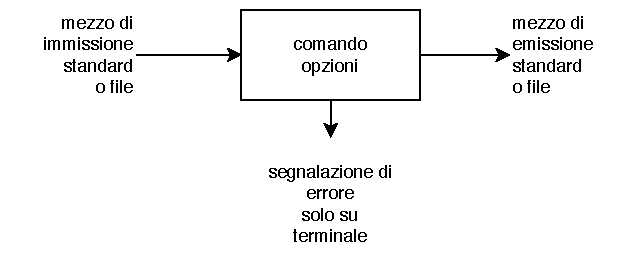
\includegraphics[height=6cm]{img/pdf/grafpag34.pdf}};
	\end{tikzpicture}
	\caption{il mezzo strandard per l'emissione del segnale è il terminale}
\end{figure}

